\documentclass[12pt,a4paper,bibliography=totocnumbered,listof=totocnumbered]{article}
\input{lib/includes}
\input{lib/commands}
\addbibresource{literatur.bib}


\begin{document}


% ----------------------------------------------------------------------------------------------------------
% Titelseite
% ----------------------------------------------------------------------------------------------------------
\newcommand{\studierenderName}{Yannic Hanel}
\student{\studierenderName}		% Studierender
{3296954}						% Matrikelnummer
{Wirtschaftsinformatik}			% Studiengang

\MyTitelseite{pics/resilent}	% Optionales Logo des extern betreuenden Unternehmens
{1}								% Style der Titelseite (1 oder 2)
{Bachelorarbeit}				% Typ der Abschlussarbeit (\in {Bachelorarbeit, Masterarbeit})
{AI-based Anomaly Detection for Electric Vehicle Supply Equipment using LSTM Architecture}				% Thema der Arbeit						
{Prof.\ Dr.\ Rudolf Hackenberg}		% Betreuer
{Prof.\ Dr.\ Sebastian Fischer}	% Zweitgutachter
{23.08.\the\year}				% Abgabedatum

%\thispagestyle{empty}
~\pagebreak

\setcounter{page}{1} 

% ----------------------------------------------------------------------------------------------------------
% Eigenständigkeitserklaerung
% ----------------------------------------------------------------------------------------------------------
\include{content/chapter/formular_stuff/erklaerung}

% ----------------------------------------------------------------------------------------------------------
% Abstract
% ----------------------------------------------------------------------------------------------------------
\thispagestyle{empty}
\setstretch{1.15} % Zeilenspacing
\section*{Abstract}

\bigskip 
This thesis explores the use of artificial intelligence for anomaly detection in electric vehicle supply equipment (EVSE), with a particular focus on wallbox charging units in private environments. The objective is to reliably detect cyberattacks and abnormal behavior by analyzing hardware and kernel event data using machine learning techniques, specifically, Long Short-Term Memory (LSTM) networks.\\
After reviewing established approaches, both publicly available datasets (hereafter referred to as CICEVSE2024) and self-collected data are analyzed, with decision trees applied for feature selection before training the LSTM models.\\
The implemented LSTM-based detection system is evaluated on both datasets and achieves high detection accuracy, especially for flooding attacks. The results demonstrate that careful feature selection significantly reduces model complexity and resource consumption, enabling real-time deployment on embedded devices. Nonetheless, limitations remain, particularly regarding cross-platform transferability and the black-box nature of LSTM models. Future work will focus on broadening the coverage of attack scenarios and extending detection to distributed, multi-station setups. Another priority will be ensuring that the detection algorithm always operates within a reserved portion of system resources. This would guarantee that Prometheus queries and anomaly detection remain functional even under severe flooding attacks.\\
Overall, this research contributes to enhancing the security and robustness of monitoring solutions for critical electric vehicle charging infrastructure.


% ----------------------------------------------------------------------------------------------------------
% contentsverzeichnis
% ----------------------------------------------------------------------------------------------------------
\titleformat{\section}{\normalfont\Large\bfseries}{\thesection}{1em}{}
\tableofcontents
\subsectionmark{} % ohne subsectionmark wird mir der content nicht angezeigt
\pagebreak

% ----------------------------------------------------------------------------------------------------------
% List of Figures
% ----------------------------------------------------------------------------------------------------------
\listoffigures

% ----------------------------------------------------------------------------------------------------------
% List of Tables (optional)
% ----------------------------------------------------------------------------------------------------------
% \listoftables


% ----------------------------------------------------------------------------------------------------------
% List of Abbreviations (optional)
% ----------------------------------------------------------------------------------------------------------
% ----------------------------------------------------------------------------------------------------------
% List of Abbreviations (optional)
% ----------------------------------------------------------------------------------------------------------
\lhead{}
\rhead{List of Abbreviations}
\listoftables
\section{List of Abbreviations}

Electric Vehicle Supply Equipment (EVSE)\\
Electric Vehicles (EVs)\\
Charging Stations (CS)\\
Artificial Intelligence (AI)\\
Isolation Forest (iForest)\\
Recurrent Neural Network (RNN)\\

\begin{acronym}[KDE]
\acro{BA}[BA]{Bachelorarbeit}
\acro{MA}[MA]{Masterarbeit}
\end{acronym}
\pagebreak

% ----------------------------------------------------------------------------------------------------------
% content
% ----------------------------------------------------------------------------------------------------------
% Format für die Überschriften
\titleformat{\section}{\normalfont\Large\bfseries}{\thesection}{1em}{}
\titleformat{\subsection}{\normalfont\large\bfseries}{\thesubsection}{1em}{}
\titleformat{\subsubsection}{\normalfont\normalsize\bfseries}{\thesubsubsection}{1em}{}

% Abstände Überschrift
\titlespacing{\section}{0pt}{12pt plus 4pt minus 2pt}{8pt plus 2pt minus 2pt}
\titlespacing{\subsection}{0pt}{12pt plus 4pt minus 2pt}{6pt plus 2pt minus 2pt}
\titlespacing{\subsubsection}{0pt}{12pt plus 4pt minus 2pt}{4pt plus 2pt minus 2pt}

% Kopfzeile
\renewcommand{\sectionmark}[1]{\markright{#1}}
\renewcommand{\subsectionmark}[1]{}
\renewcommand{\subsubsectionmark}[1]{}
\lhead{Chapter \thesection}
\rhead{\rightmark}

%\onehalfspacing
\setstretch{1.15}
\renewcommand{\thesection}{\arabic{section}}
\renewcommand{\theHsection}{\arabic{section}}
\setcounter{section}{0}
\pagenumbering{arabic}
\setcounter{page}{1}


% ----------------------------------------------------------------------------------
% Kapitel: introduction 5
% ----------------------------------------------------------------------------------
\section{Introduction}
\subsection{Motivation and Relevance of Anomaly Detection in Electric Vehicle Supply Equipment}

Electric Vehicle Supply Equipment (EVSE) has gained significant importance in recent years \cite{paper_relevance_EVSE}. Analyzing the market sales of electric vehicles (EVs), a remarkable growth can be observed. In 2012, only 120,000 EVs were sold, whereas by 2021, sales had surged to nearly 6.6 million. To achieve net-zero CO2 emissions by 2050, as planned by the European Union \cite{EU2050}, the number of EVs must continue to rise substantially, requiring an 11-fold increase from current levels by 2030 \cite{Number_of_EVSE_sales}.\\
To manage the much higher demand for EVs on public roads, it is expected that the market for EVSE will grow similarly to the sales of EVs \cite{ladeinfrastruktur}. The correlation between the number of EVs and the number of EVSE is high. Market data from the last few years show that the top four countries in the European Union, such as Germany, the Netherlands, France, and Belgium, with the best EVSE infrastructure, are also the top four with the largest market share of EVs \cite{ladeinfrastruktur}.
\begin{figure}[htbp]
  \centering
  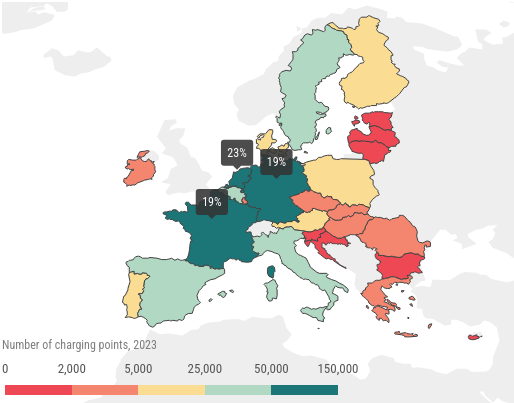
\includegraphics[width=0.5\textwidth]{pics/chargingPointsInfrastructure.png}
  \caption{Availability of public charging points and market share of electric cars in the European Union \cite{ladeinfrastruktur}.}
  \label{fig:chargingPointsInfrastructure}
\end{figure}
\\
With the growing number of EVSE, particularly Charging Stations (CS), the interest of cyber-criminal groups in attacking these systems is also increasing \cite{silicon_evse_attacks}. At first glance, EVSE systems may not appear to be direct targets for accessing critical data or manipulation. Upon closer examination, it turns out that they can serve as entry points to gain access to more sensitive or private information \cite{nature2025}. The following figure illustrates how EVSE components, such as charging stations, can act as access nodes to critical or private data.
\begin{figure}[H]
  \centering
  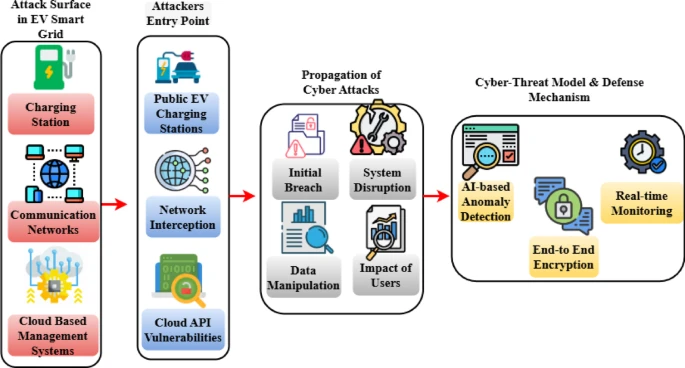
\includegraphics[width=0.7\textwidth]{pics/EVSE_attackpoints.png}
  \caption{Electric Vehicle Supply Equipment as an access node to critical data \cite{nature2025}.}
  \label{fig:EVSE_attackpoints}
\end{figure}

With access to these kinds of data, critical attacks, such as data manipulations, data theft, disruption of service, or even complete system failure, are possible \cite{nature2025}. This does not only lead to a high financial risk, but it also affects the trust of users in EVSE systems and potentially slows down the adoption of EVs in general.\\
If end users are provided with a stable and secure EVSE infrastructure, consumer confidence in switching to electric vehicles will be significantly higher. This ensures, in turn, consistent growth in the adoption of both EVs and EVSE systems \cite{evse-cybersecurity2025}.\\
As outlined in the first paragraphs, the rapid growth of EVs and EVSE infrastructure also requires a robust monitoring and anomaly detection system to safeguard the security of the EVSE infrastructure. Only by guaranteeing a secure EVSE environment can user trust in the energy transition be maintained and major cybersecurity incidents in the future be avoided.\\

Ensuring high security standards for EVSE systems is of critical importance, but difficult to achieve. The EVSE infrastructure constitutes a complex system that includes not only charging stations but also sophisticated backend systems and communication protocols. These components and software solutions are typically developed, published, and maintained by various vendors, which makes securing the entire system a challenging task.\\
Combining all the different software from vendors into a secure infrastructure is challenging enough, but the EVSE infrastructure, especially charging stations (CS), is also regularly installed in public places. Even when not in a public setting, these installations are often outdoors, where security measures are significantly lower than in buildings protected by walls, doors, and other physical barriers.\\
In this paper, the focus is on wallboxes, which are generally smaller than CS and are typically used in private settings. They are often installed directly on house walls or in garages, and thus still form part of the overall EVSE infrastructure.\\
The fact that they are installed in private areas initially suggests a higher level of security. However, since these areas are still outdoors, it must be assumed that there are no additional physical security measures beyond the wallbox itself. It is crucial to develop a system that not only protects against software-based attacks, such as Denial-of-Service (DoS) or Distributed Denial-of-Service (DDoS), but also considers other potential attack vectors, such as firmware manipulation and unauthorized data interception. In addition, the system has to secure the hardware against physical threats, like tampering, theft, or other intrusions.\\

In this project, wallboxes from the \textit{ReSiLENT} \cite{ReSiLENT} project, provided by \textit{Stöhr Mobility GmbH} \cite{StoehrMobility}, are used. The software is developed by \textit{ChargeIQ GmbH} \cite{ChargeIQ} and already includes basic security measures to protect against external threats. This project is also carried out in cooperation with \textit{ASVIN GmbH} \cite{ASVIN}. In the following chapter, the internal components of the wallbox are examined more closely.\\

\begin{figure}[H]
  \centering
  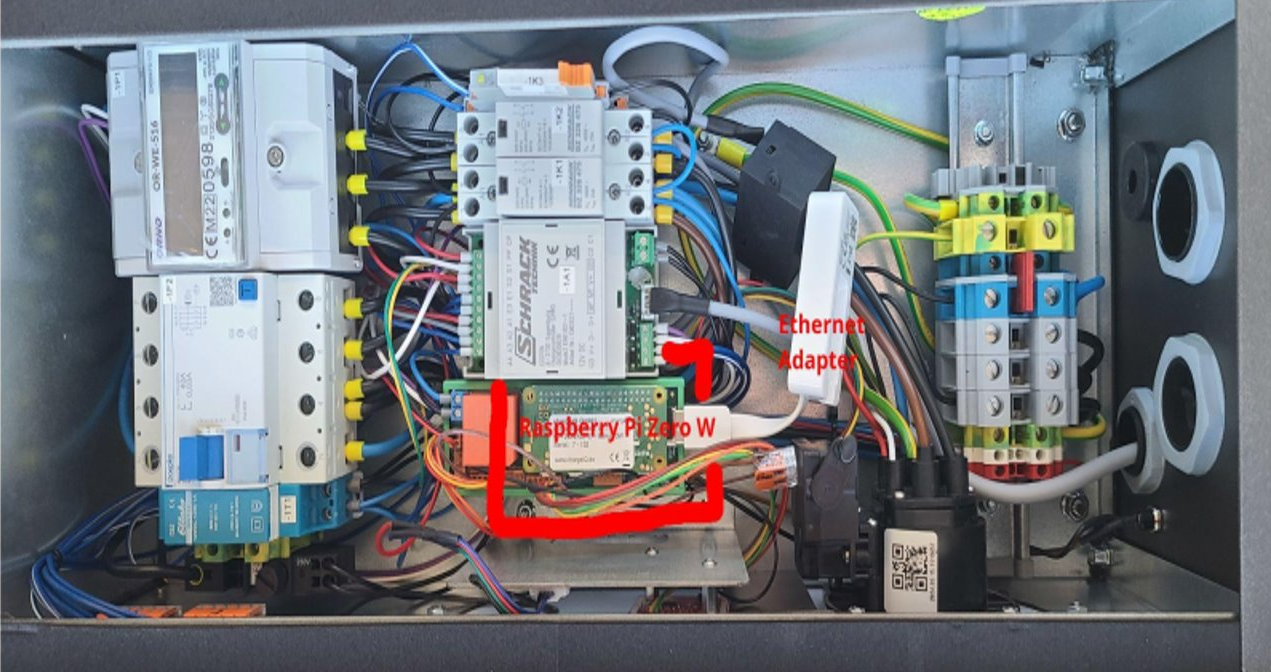
\includegraphics[width=0.7\textwidth]{pics/wallbox.png}
  \caption{Interior view of the wallbox \cite{wallbox}.}
  \label{fig:Wallbox}
\end{figure}

In this figure, the internal components of the wallbox are visible. The wallbox is equipped with a Raspberry Pi Zero W, which is responsible for communication with the backend, including the transmission of user data and handling of payment processes from the charging process. This component is secured and programmed by \textit{ChargeIQ GmbH} \cite{ChargeIQ}.\\
The sensitive hardware components are enclosed in an aluminum casing designed by \textit{Stöhr Mobility GmbH} \cite{StoehrMobility}, which provides a degree of protection against physical attacks.\\
As already mentioned, the wallbox also processes personal data of users, such as their user ID and payment information, in communication with the backend server. This requires special attention in the context of the DSGVO / GDPR, as additional requirements for the protection of personal data, such as data minimization, storage limitation \cite{DSGVOart5}, and legal obligation \cite{DSGVOart6}, must be taken into account throughout the entire EVSE infrastructure.\\

Security requires significant computational resources, particularly in the domain of anomaly detection. As shown in Figure~\ref{fig:Wallbox}, the wallbox is equipped with a Raspberry Pi Zero W, which offers sufficient resources for a single-board computer. However, when processing and analyzing over 900 hardware events to detect potential anomalies, the system quickly reaches the limits of its hardware capabilities. This is just a small example of the challenges faced in securing EVSE infrastructure.\\
Due to the combination of digital and physical threats, the involvement of multiple vendors, and strict data protection requirements, securing Electric Vehicle Supply Equipment (EVSE) infrastructure is a complex task and entails numerous challenges.
\subsection{Overview of Artificial Intelligence-based Approaches}

Artificial intelligence is often used in different contexts; therefore, it is necessary to define what is meant by AI-based approaches and which different approaches exist. It is a leading technology in the current digital transformation and is crucial for advancing the fourth industrial revolution \cite{AI-Definition}.\\
The goal of AI is to create machines that can perform tasks that typically require human intelligence, such as understanding natural language and recognizing patterns in data. In particular, the detection of patterns is of relevance in this work. The different AI-based approaches can be divided into two subcategories \cite{AI-Definition}:
\begin{figure}[H]
  \centering
  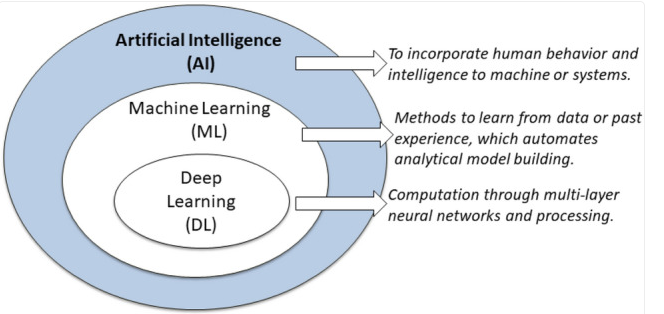
\includegraphics[width=0.7\textwidth]{pics/AI_approaches.png}
  \caption{An illustration of the position of Machine Learning and Deep Learning within the area of Artificial Intelligence \cite{AI-Definition}}
  \label{fig:AI_approaches}
\end{figure}
These can be further divided into three categories:
\begin{itemize}
  \item \textbf{Supervised Learning:} This approach involves learning from labeled data to identify patterns and make predictions. It is commonly used in tasks such as email spam classification or price prediction, where the algorithm is trained on known input-output pairs.
  \item \textbf{Unsupervised Learning:} This data-driven method is used to uncover hidden patterns in unlabeled data. Techniques such as clustering and dimensionality reduction are applied to identify structures within the data, for example, to segment customer groups or discover business models.
  \item \textbf{Semi-Supervised Learning:} This approach combines aspects of both supervised and unsupervised learning by utilizing a small amount of labeled data alongside a larger pool of unlabeled data. It is particularly useful when labeling data is expensive or time-consuming, but large amounts of unlabeled data are available.\\
\cite{AI-Definition}\\
\end{itemize}

In the following table, the different approaches are categorized alongside their corresponding machine learning architectures. This allows identification of the advantages and disadvantages of each method and provides a clearer understanding of which approach is most suitable for producing actionable results in real-world deployments.
\begin{table}[H]
	\centering
	\begin{tabular}{|l|p{3.5cm}|p{4cm}|p{4cm}|}
		\hline
		\textbf{Approach} & \textbf{Examples} & \textbf{Advantages} & \textbf{Disadvantages}\\
		\hline
		Supervised Learning & Decision Trees, \newline Random-Forest, \newline LSTM & High prediction accuracy, \newline Clear objectives & Requires a lot of labeled data, \newline Risk of overfitting\\
		\hline
		Unsupervised Learning & K-Means, \newline Isolation-Forest & Finds patterns without labels, \newline Useful for unlabeled data & Hard to interpret, \newline No clear target\\
		\hline
		Semi-Supervised Learning & Self-training & Improves performance with few labeled data points & Complex to implement\\
		\hline
	\end{tabular}
	\caption{Comparison of machine learning approaches with examples, advantages, and disadvantages \cite{AI-Definition}.}
    \label{tab:AI_approaches}
\end{table}

After providing an overview of the different machine learning approaches, the following chapter delves deeper into the field by examining various methods for anomaly detection and identifying the most effective models for detecting typical anomalies.

\subsection{Research Questions}

The following research questions guide this thesis on \textbf{AI-based Anomaly Detection for Electric Vehicle Supply Equipment using LSTM Architecture}:

\begin{itemize}
    \item What types and characteristics of anomalies occur in electric vehicle supply equipment (EVSE)?
    \item How can relevant features be identified and selected to effectively train machine and deep learning models for anomaly detection?
    \item How does the performance of LSTM-based models compare to that of traditional or alternative AI-based methods in terms of detection accuracy and false positives?
    \item What practical challenges arise when implementing such anomaly detection systems in real-world charging infrastructure?
\end{itemize}

These research questions address both the technical and real-world aspects of developing and applying anomaly detection, providing the analytical framework for the subsequent chapters of this thesis.

\subsection{Structure of the Thesis}
This thesis is divided into ten chapters, each building upon the previous to explore the use of AI-based methods—specifically LSTM architectures—for anomaly detection in Electric Vehicle Supply Equipment (EVSE).\\
Chapter~1 introduces the motivation and relevance of the topic, outlines the role of anomaly detection in the context of EV infrastructure, and formulates the central research questions. Additionally, it provides an overview of prior AI-based approaches and concludes with this structural outline. Chapter~2 summarizes the key theoretical foundations necessary for the thesis, including the basics of anomaly detection, a short introduction to tree-based models such as decision trees and random forests, and a focused explanation of the LSTM architecture.\\
Chapter~3 presents related work, covering research on security aspects and anomaly detection mechanisms specific to EVSE, as well as a broader review of AI-based detection methods applied in similar domains. Chapter~4 describes the dataset creation and acquisition process, detailing both public datasets and custom setups involving Prometheus monitoring tools. Chapter~5 follows with an exploratory data analysis (EDA), intended to uncover key patterns and differences between the public and self-generated datasets.\\
In Chapter~6, the process of data preprocessing and feature selection is discussed, including the identification of relevant features and the use of feature importance methods such as decision trees. Chapter~7 focuses on the LSTM model itself, describing its architecture, the training process, and the chosen strategies for hyperparameter tuning. \\
The results of the approach are then evaluated in Chapter~8, which outlines the experimental setup, evaluation metrics, and key results of the applied anomaly detection system. Chapter~9 provides a detailed discussion of the findings in relation to the research questions, highlighting limitations and potential practical applications. Finally, Chapter~10 concludes the thesis with a summary of the work and a reflection on future directions.\\
This structure ensures a logical and methodical development of the topic, from theoretical foundations to implementation, evaluation, and critical interpretation.



\pagebreak
% ----------------------------------------------------------------------------------
% Kapitel: Fundamentals and Key Terminologies 5
% ----------------------------------------------------------------------------------
\section{Fundamentals and Key Terminologies}
% ----------------------------------------------------------------------------------
% Kapitel: Fundamentals and Key Terminologies 5
% ----------------------------------------------------------------------------------
\subsection{Fundamentals of Anomaly Detection}
In the previous chapter, a closer look was taken at what Artificial Intelligence is and how useful it can be in the field of EVSEs. In this chapter, the focus is on the area of Anomaly Detection and its fundamental concepts.\\
Anomaly Detection is the process of analyzing data patterns to identify outliers. Data points deviate significantly from the norm. This technique can be applied in a wide range of domains, including credit card fraud detection, insurance and healthcare monitoring, intrusion detection in cybersecurity, fault detection in safety-critical systems, military surveillance, and also in the field of EVSEs \cite{paper_AnomalyDetection_Northwestern}.\\
Outliers are data points that differ significantly from the majority of the data. In the paper by Hodge and Austin, they define outliers as "data points that are inconsistent with the rest of the data". The paper also includes some informative figures that illustrate the different types of outliers and how they can be detected \cite{paper_HodgeAustin}.\\
\begin{figure}[H]
  \centering
  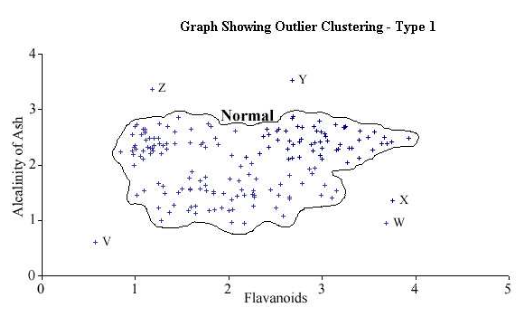
\includegraphics[width=0.5\textwidth]{pics/outlier_clustering_type1.png}
  \caption{Data distribution classified by Type 1: Outlier Clustering \cite{paper_HodgeAustin}.}
  \label{fig:outlier_clustering_type1}
\end{figure}
Type 1 is the most common form of outlier, data points are generally clustered around a central value, but a few points differ significantly from the rest. This can be seen in the Figure~\ref{fig:outlier_clustering_type1}, where most data is centered, yet a few outliers deviate clearly.\\
Such outliers can be detected using a simple Z-score algorithm, where the mean $\mu$ and the standard deviation $\sigma$ of the data are calculated. The Z-score is computed using the formula: $Z = \frac{X - \mu}{\sigma}$. Estimated Z-scores greater than 3 or less than -3 can be considered anomalies. These anomalies should be given increased attention during data analysis. Additionally, anomalies can be contextualized by parameters such as time or location to improve their identification \cite{paper_IJITEE_z_score}.
\begin{figure}[H]
  \centering
  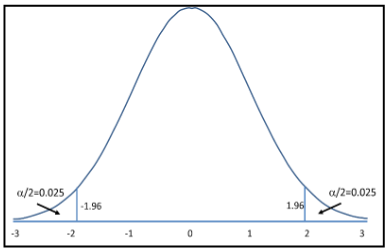
\includegraphics[width=0.4\textwidth]{pics/z_score.png}
  \caption{Z-score with critical region \cite{paper_IJITEE_z_score}}
  \label{fig:z_score}
\end{figure}
Before the Z-score can be calculated, extensive data collection and preprocessing are required. This forms the first step in the Anomaly Detection process. The data must be cleaned, normalized, and transformed to ensure that its suitable for analysis. This may involve removing duplicates, handling missing values, and scaling the data to a common range.\\
After the data is preprocessed, feature engineering is performed to extract relevant features from the data. Feature engineering involves selecting and transforming the data and can sometimes also include the creation of new features that improve the performance of the anomaly detection model. Data reduction is also a relevant step in this process, where the data is reduced to a smaller set of features that are most relevant for the anomaly detection task \cite{maharana2022review}.\\
Once data collection and preprocessing are completed, a suitable model must be selected for the specific anomaly detection case. Before analyzing the different models, it is important to examine the typical challenges associated with anomaly detection.\\
As previously mentioned, detecting anomalies requires analyzing data patterns to identify outliers. Determining the correct boundary between normal and abnormal data is challenging and highly dependent on the context.\\
The EVSE infrastructure changes rapidly. This happens not only due to new technologies, charging stations also change with every new charging process and through communication with other stations in the network. This variability makes it difficult to define a static outlier threshold. Therefore, it is essential to adapt the anomaly detection model to the current state of the EVSE network and the ongoing charging processes. This enables dynamic detection capabilities that remain effective under all conditions in a highly dynamic EVSE environment \cite{paper_AnomalyDetection_Northwestern}.\\

\subsection{introduction to Decision Trees, Random Forest, Isolation Forest and LSTM}
In this section, we will provice a brief introduction to serveral machine learning models who are categorized as supervised learningn models. These models are also the most relevant for our project.\\
The \textbf{Decision tree} classifiers are the most well known and one of the powerful models in various fileds. It works by creating a tree-like strucutere with Nodes and Branches and every Node is an Attribute or feature and the Branch can referent the characteristic of the Attribute\cite{decision_tree_explain}. 
\begin{figure}[H]
  \centering
  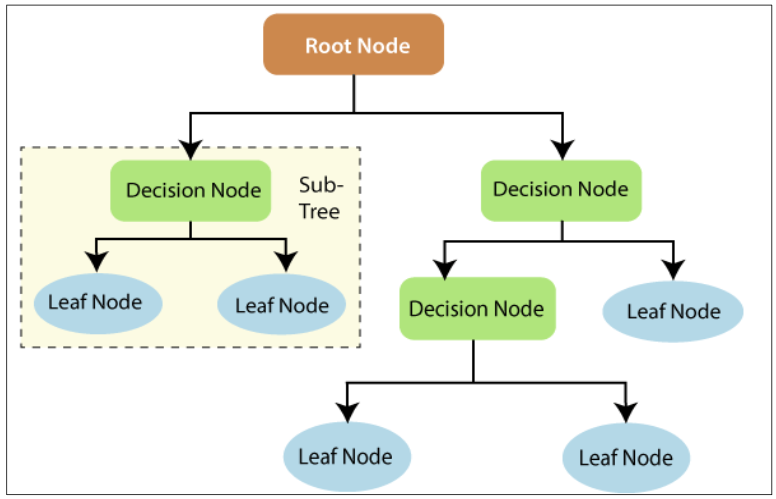
\includegraphics[width=0.5\textwidth]{pics/decision_tree_explain.png}
  \caption{Decision Tree\cite{decision_tree_explain}}
  \label{fig:decision_tree}
\end{figure}
The decision rule is not a black box and can be easily interpreted. It compares the value of the feature with a threshold and then decides which branch to follow. It is not only used in Machine Learning, but is also common in fields like image processing and pattern recognition, due to its simple analysis and high accuracy. Despite these advantages, it has a high risk of overfitting, especially with small datasets.\cite{decision_tree_explain}\\
The \textbf{Random Forest} is an ensemble method that combines multiple decision trees that work independently of each other. Each decision tree is created using a random vector to improve variance and reduce overfitting.\\
The final decision is made by majority vote of all the trees together. This method is more robust against overfitting and can handle large datasets with high dimensionality. Two key vectors influence the performance of the Random Forest: the correlation between the trees and the strength of the individual trees.\cite{breiman2001randomforests}\\
The \textbf{Isolation Forest} is an innovative approach for anomaly detection. While conventional methods typically create a model of "normal" behavior and classify deviations from it as anomalies, the iForest follows the principle of directly isolating anomalies.\cite{iForest}\\
The explanation for this is that anomalies are characterized by their rarity and by being significantly different in their attributes. Therefore, they are easier to separate from the majority.\\
This model brings advantages such as robustness with regard to dimensionality and irrelevant features. On the other hand, \textit{swamping} is one of the disadvantages, where normal instances that are too close to anomalies can prevent anomalies from being isolated and thus make them harder to detect.\cite{iForest}\\
A \textbf{Long Short-Term Memory (LSTM)} is a special type of Recurrent Neural Network (RNN) designed to model sequential data and long-term dependencies. Especially the long-term dependencies have high priority in this project, where the focus is on detecting anomalies over longer time periods. LSTMs use memory cells and gating mechanisms to store information over long time steps reliably. Despite their many advantages, they come with many different parameters, making them difficult to tune. Additionally, they represent a black-box model, meaning it is hard to understand why the model made a certain decision.\cite{LSTM_understanding}\\
\begin{table}[H]
	\centering
	\begin{tabular}{|l|p{4cm}|p{4cm}|}
		\hline
		\textbf{Machine Learning Model} & \textbf{Advantages} & \textbf{Disadvantages} \\
		\hline
		Decision Tree & Easy to understand and interpret & High possibility of overfitting \\
		\hline
		Random Forest & Less overfitting than a single decision tree; handles high-dimensional data & Not well-suited for small datasets \\
		\hline
		Isolation Forest & Robust to high-dimensional and irrelevant features & Swamping effect in presence of nearby normal instances \\
		\hline
        Long Short-Term Memory & Effective at modeling long-term dependencies & Black-box nature and complex parameter tuning \\
		\hline
	\end{tabular}
	\caption{Comparison of supervised learning models with advantages and disadvantages. Own illustration based on \cite{decision_tree_explain}\cite{breiman2001randomforests}\cite{iForest}\cite{LSTM_understanding}.}
    \label{tab:supervised_learning_models}
\end{table}
\subsection{Overview of LSTM (Long Short-Term Memory) Architecture}




\pagebreak
% ----------------------------------------------------------------------------------
% Kapitel: Related Work 2
% ----------------------------------------------------------------------------------
\section{Related Work}
\subsection{Recent Advances in Cybersecurity and Anomaly Detection for Electric Vehicle Supply Equipment}

In the emerging field of EVSE, numerous studies focus either on electric vehicle supply equipment itself or on anomaly detection methods. However, the specific combination of anomaly detection applied to EVSE is not yet widely explored. Therefore, the paper \cite{EV_Security}, titled "Enhancing EV Charging Station Security Using a Multi-dimensional Dataset", is highly relevant to this research. The authors present a dataset used for anomaly detection that includes similar features such as hardware events, power consumption, and other HPC-related data. The paper focuses on various attack scenarios and attempts to detect them using several machine learning models.\\
\\
Another relevant contribution in this field is the paper \cite{paper_relevance_EVSE}, titled "Regression-Based Anomaly Detection in Electric Vehicle State of Charge Fluctuations Through Analysis of EVCI Data" which not only highlights the importance of anomaly detection in EVSE but also provides a comprehensive overview of a realistic charging station scenario. The setup includes four different charging boards, six charging ports, and a battery energy storage system (BESS) handling various types of EVs. The study monitors the state-of-charge (SoC) values of EVs, compares them with expected values, and detects outliers that may indicate anomalies. These detections are performed using machine learning methods within a dynamic environment.\\
\\
In the context of EVSE as part of critical infrastructure, recent research highlights its role as a potential attack vector within complex smart grid environments. Studies report threats such as Denial-of-Service (DoS), Man-in-the-Middle (MitM), spoofing, and data manipulation. Modern approaches increasingly integrate anomaly detection methods using machine learning to identify and mitigate such attacks at an early stage. While not all technical implementation details are relevant here, the findings emphasize the need for advanced security mechanisms to ensure the integrity and availability of EVSE systems \cite{nature2025}.

\subsection{Performance Comparison of Deep Learning Approaches for EVSE Anomaly Detection}

In the following, it is important to summarize which machine learning and deep learning algorithms have shown promising performance in the field of anomaly detection for EVSE. Since the data involves time series and hardware-related measurements, the paper \cite{deeplearing_compare_EVSE}, titled \textit{Deep Learning-based Intrusion Detection System for Electric Vehicle Charging Station}, provides a valuable overview of suitable deep learning models in this context.\\
The authors compare a Deep Neural Network (DNN) with a Long Short-Term Memory (LSTM) model and conclude that the LSTM architecture achieves high accuracy—over 99\%—after only a few training epochs. This supports the later decision in this thesis to select the LSTM model for better performance and anomaly detection in EVSE environments.\\
\\
But the LSTM is only as strong as the significance of its features. Therefore, a good feature selection for the LSTM algorithm is essential to achieve an effective deep learning approach for anomaly detection. The paper by Kottilingal (2024) \cite{feature_selection} offers a systematic comparison of different feature selection methods in combination with an LSTM network for intrusion detection. The authors evaluate both the detection accuracy and the efficiency of the LSTM model when applying various feature selection strategies. The central finding is that reduced feature sets—such as those selected using tree-based methods—can achieve almost the same detection accuracy as larger sets, while significantly lowering model complexity and computational requirements. This aspect is particularly relevant for resource-constrained environments such as embedded EVSE systems.\\
In the context of EVSE, this means that implementing a practical and high-performance anomaly detection system requires not only choosing a suitable deep learning model (e.g., LSTM) but also effectively reducing the input dimensionality through feature selection. As already shown in \cite{EV_Security}, even with EVSE-specific data, selecting a smaller but relevant subset of hardware and kernel events can maintain detection accuracy while significantly reducing system load. The work by Kottilingal supports this approach with experimental results and provides practical recommendations for combining deep learning architectures with feature selection, making it a valuable reference for objective method comparisons in smart charging anomaly detection.


\pagebreak
% ----------------------------------------------------------------------------------
% Kapitel: Data Acquisition 9
% ----------------------------------------------------------------------------------
\section{Data Acquisition}
\section{Data Acquistion}
\subsection{Description of Data Sources for EVSE Anomaly Detection}
\subsection{Integration of Prometheus}  
In the research on which database would be suitable for centralized data storage and analysis, Prometheus played a central role. Not only is it an open-source project \cite{prometheus_wiki}, but it is also well known in the industry as a reliable monitoring solution for complex systems. It has a large community, along with comprehensive documentation and strong support, which are essential for maintaining a stable IT environment.\\
Another reason for choosing Prometheus is its seamless integration with Grafana for visualization, as well as its powerful PromQL query language. Additionally, Prometheus can store metrics in a time series database, which is particularly important for the detection systems \cite{prom_advantages}.\\

Prometheus consists of several components that are required for its operation. The core of the system is the Prometheus server, which collects and stores metrics and provides access to them through the Prometheus Query Language (PromQL).\\
Client libraries are directly integrated into the application code and expose a client-server interface. The Prometheus server periodically fetches data from them, by default every 15 seconds, this interval is configurable \cite{Prometheus_how_it_works}.\\

As explained in the previous subsection, Prometheus collects data via metrics exporters \ref{lst:perf-prometheus-exporter}. After the data is collected and stored centrally in the Prometheus time series database, a Python script was developed that allows exporting the data within a defined time range and with specified time steps.\\
This export functionality is essential for enabling further analysis, including exploratory data analysis, using external tools such as Python or statistical software. The following paragraph presents the Python script developed to export Prometheus data into a structured \texttt{CSV} format, enabling its direct use in subsequent analytical workflows.\\

The Python script is designed to systematically retrieve and organize time-series metrics from a Prometheus monitoring server, facilitating subsequent analysis and interpretation. The workflow begins by defining a specific time range for the data of interest and partitioning this interval into smaller, manageable chunks, which helps prevent overwhelming the server with excessively large queries and ensures efficient data retrieval. For each feature specified in an external configuration file, the script constructs appropriate Prometheus queries, attempting first to obtain the standard metric and, if unavailable, a performance-prefixed variant. The retrieved data are then parsed and organized according to their respective timestamps, forming a structured representation of the system's behavior over time. Finally, the script outputs these metrics in a wide-format \texttt{CSV} file, where each row corresponds to a timestamp and each column corresponds to a specific metric. This approach not only allows for straightforward integration with downstream data analysis or visualization workflows but also ensures reproducibility, scalability, and clarity in the presentation of high-dimensional monitoring data.




\pagebreak
% ----------------------------------------------------------------------------------
% Kapitel: Exploratory Data Analysis 5
% ----------------------------------------------------------------------------------
\section{Exploratory Data Analysis}
\section{Exploratory Data Analysis}
\subsection{Exploratory Data Analysis in the Context of EVSE Anomaly Detection}
\subsection{Comparison of Public and Self-Generated Datasets}
% warum ist der Vergleich wichige? zwischen den beiden Datensätzen
The paper \textit{Enhancing EV Charging Station Security Using a Multi-dimensional Dataset}~\cite{EV_Security} and my work pursue the same goal: detecting anomalies through the analysis of HCP and kernel events. Therefore, it is essential to compare the underlying datasets on which the machine learning algorithms are trained. Such a comparison enables validation of the respective approaches and helps determine whether the results can be generalized.

% Beschreibung der Datensaätze: Herkunft Umfang, Struktur, Einschrnänkunen
We tried to get as close as possible to the environment of the paper \textit{Enhancing EV Charging Station Security Using a Multi-dimensional Dataset}\\
\begin{figure}[H]
  \centering
  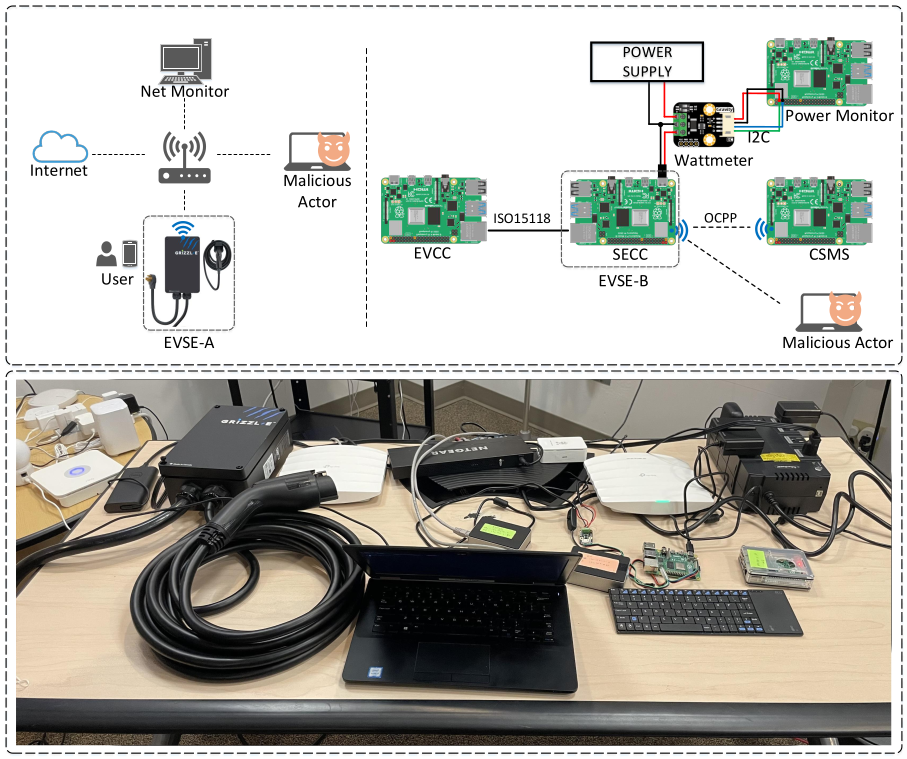
\includegraphics[width=0.7\textwidth]{pics/setup_public_paper.png}
  \caption{setup EV Charing Station from \cite{EV_Security}}
  \label{fig:setup_public_paper}
\end{figure}
We also used a Raspberry Pi to represent the EVSE-B and employed a wattmeter to monitor power consumption. The combination of HCP events, kernel events, and power consumption measurements will be discussed in future work. As mentioned in Chapter~\texttt{Data Sources for EVSE Anomaly Detection}, we also used the \texttt{perf} tool to monitor the various events.\\
\\
Therefore, we are able to observe approximately 900 events—similar to the comparison dataset. The complete observation period spans from \texttt{2025-07-22T18:00:00} to \texttt{2025-07-23T12:52:10}, with a sampling interval of 10 seconds, resulting in approximately 8,000 data rows with 905 columns. There are no missing (NaN) values in the dataset, and all measurements were collected using the \texttt{perf} tool, producing logically consistent outputs, as described in the chapter \textit{Data Sources for EVSE Anomaly Detection}.\\
Features that are distributed across multiple CPU cores (e.g., \texttt{cpu=0,1,2,3}) are aggregated using appropriate \texttt{perf} flags. This prevents data loss and reduces the number of distinct features, aligning the dataset structure more closely with that of the comparison \texttt{CICEVSE2024} dataset.\\
The \texttt{CICEVSE2024} dataset consists of the same 905 event types and comprises approximately 8,500 rows. Timestamps are recorded as floating-point numbers representing the time of each measurement. The data was collected using the \texttt{perf} tool, ensuring high precision and consistency across all recorded events.\\
Out of the entire dataset, only four rows contain \texttt{NaN} values across all features. These rows can be considered outliers or errors and can easily be excluded during preprocessing. To ensure comparability with the reference dataset, features distributed across multiple CPU cores (e.g., \texttt{cpu=0,1,2,3}) were aggregated using appropriate \texttt{perf} flags. While it is not explicitly stated in the documentation of the \texttt{CICEVSE2024} dataset whether a similar aggregation was performed, the reduced feature dimensionality suggests that such a step may have been taken. Therefore, this approach was adopted in our dataset to align the structure and avoid data duplication.
% Visulaisierung der Unterschiede
\begin{figure}[H]
  \centering
  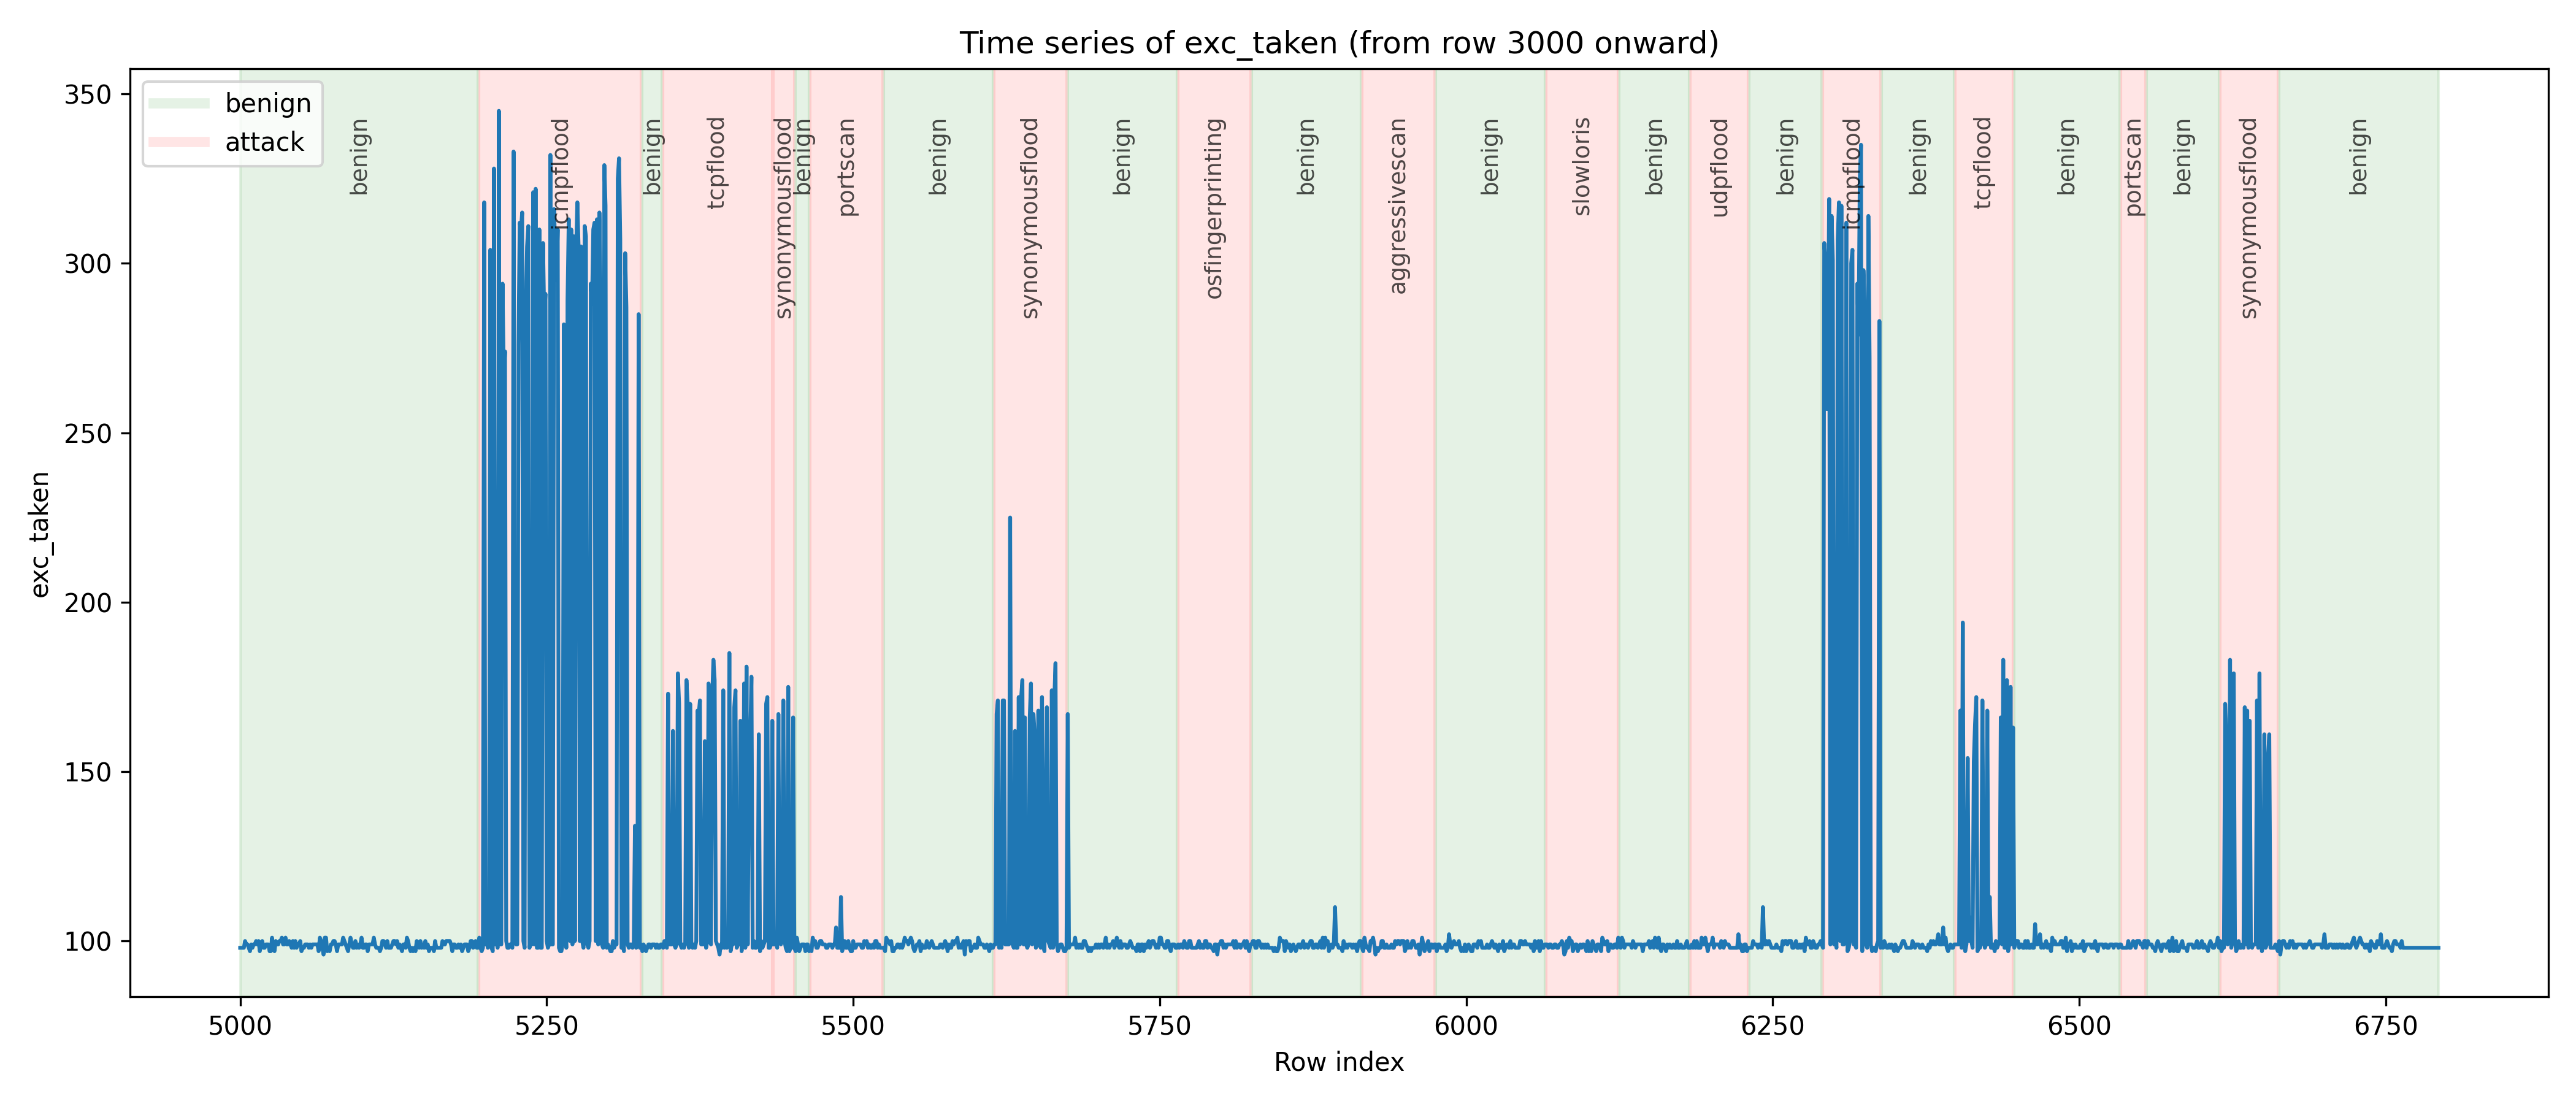
\includegraphics[width=1\textwidth]{pics/exc_taken.png}
  \vspace{-3mm} % Abstand manuell entfernen (anpassbar)
  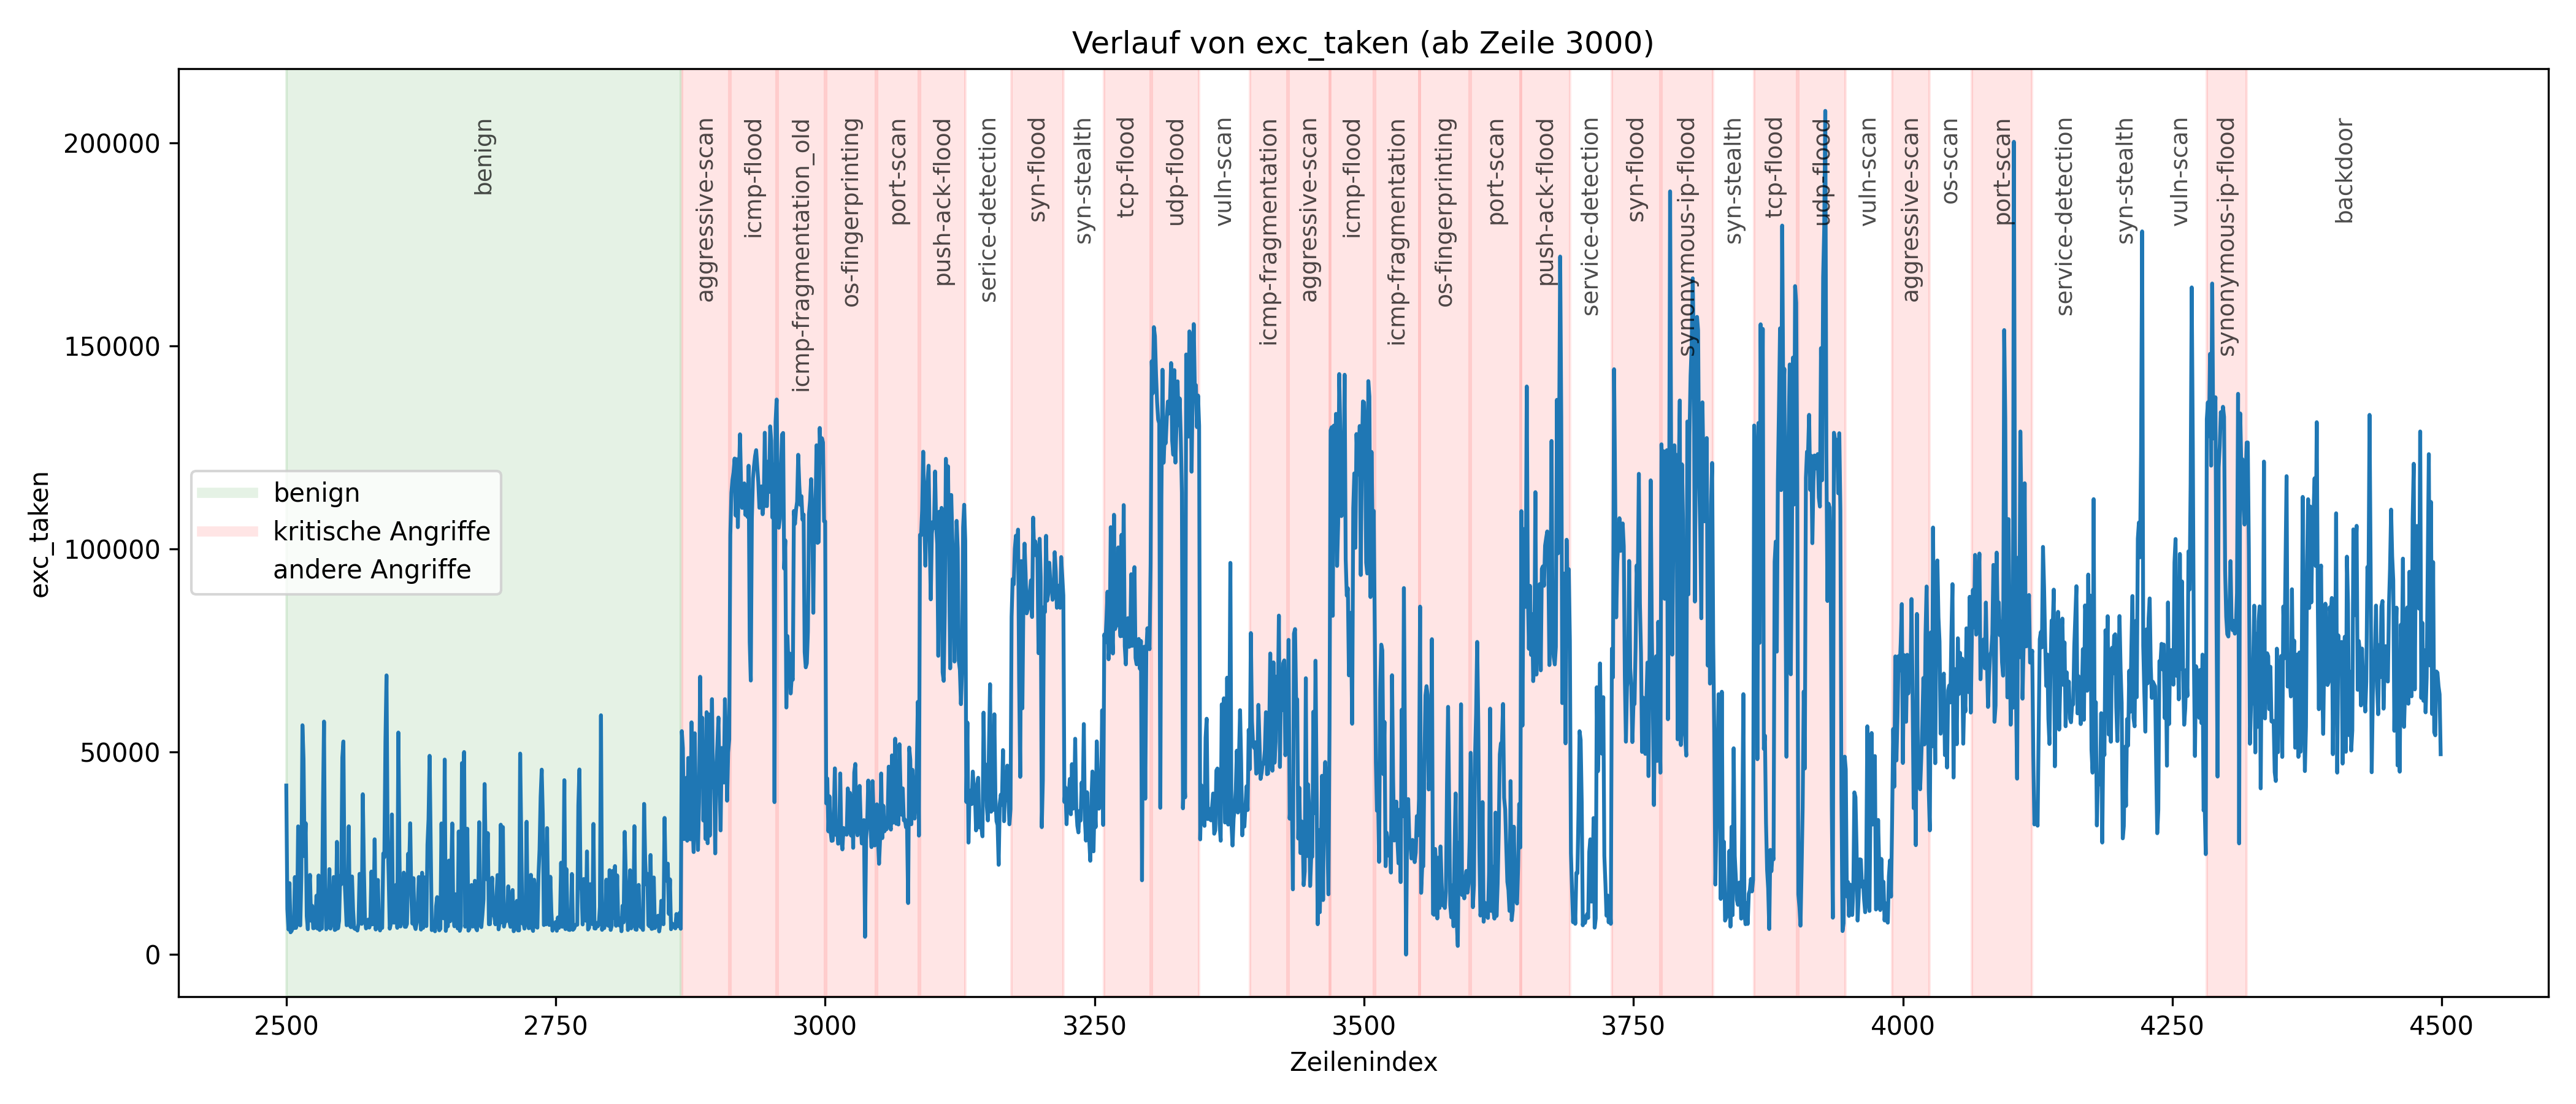
\includegraphics[width=1\textwidth]{pics/exc_taken_public.png}
  \caption{Comparison of \texttt{exc-taken} timelines: own dataset (top) and CICEVSE2024 dataset (bottom)}
  \label{fig:exc_taken_comparison}
\end{figure}
Despite notable differences in the absolute value ranges—likely due to architectural differences, sampling intervals, and system load—the time series of \texttt{exc\_taken} in both datasets exhibit structurally similar patterns. In both cases, this feature reacts to specific attacks with abrupt value changes especially by the flooding attacks are distinctive spikes, while maintaining stable behavior during benign phases. This confirms \texttt{exc\_taken} as a sensitive and transferable indicator of anomalous activity in kernel-space, suitable for machine learning-based intrusion detection approaches.
\begin{figure}[H]
  \centering
  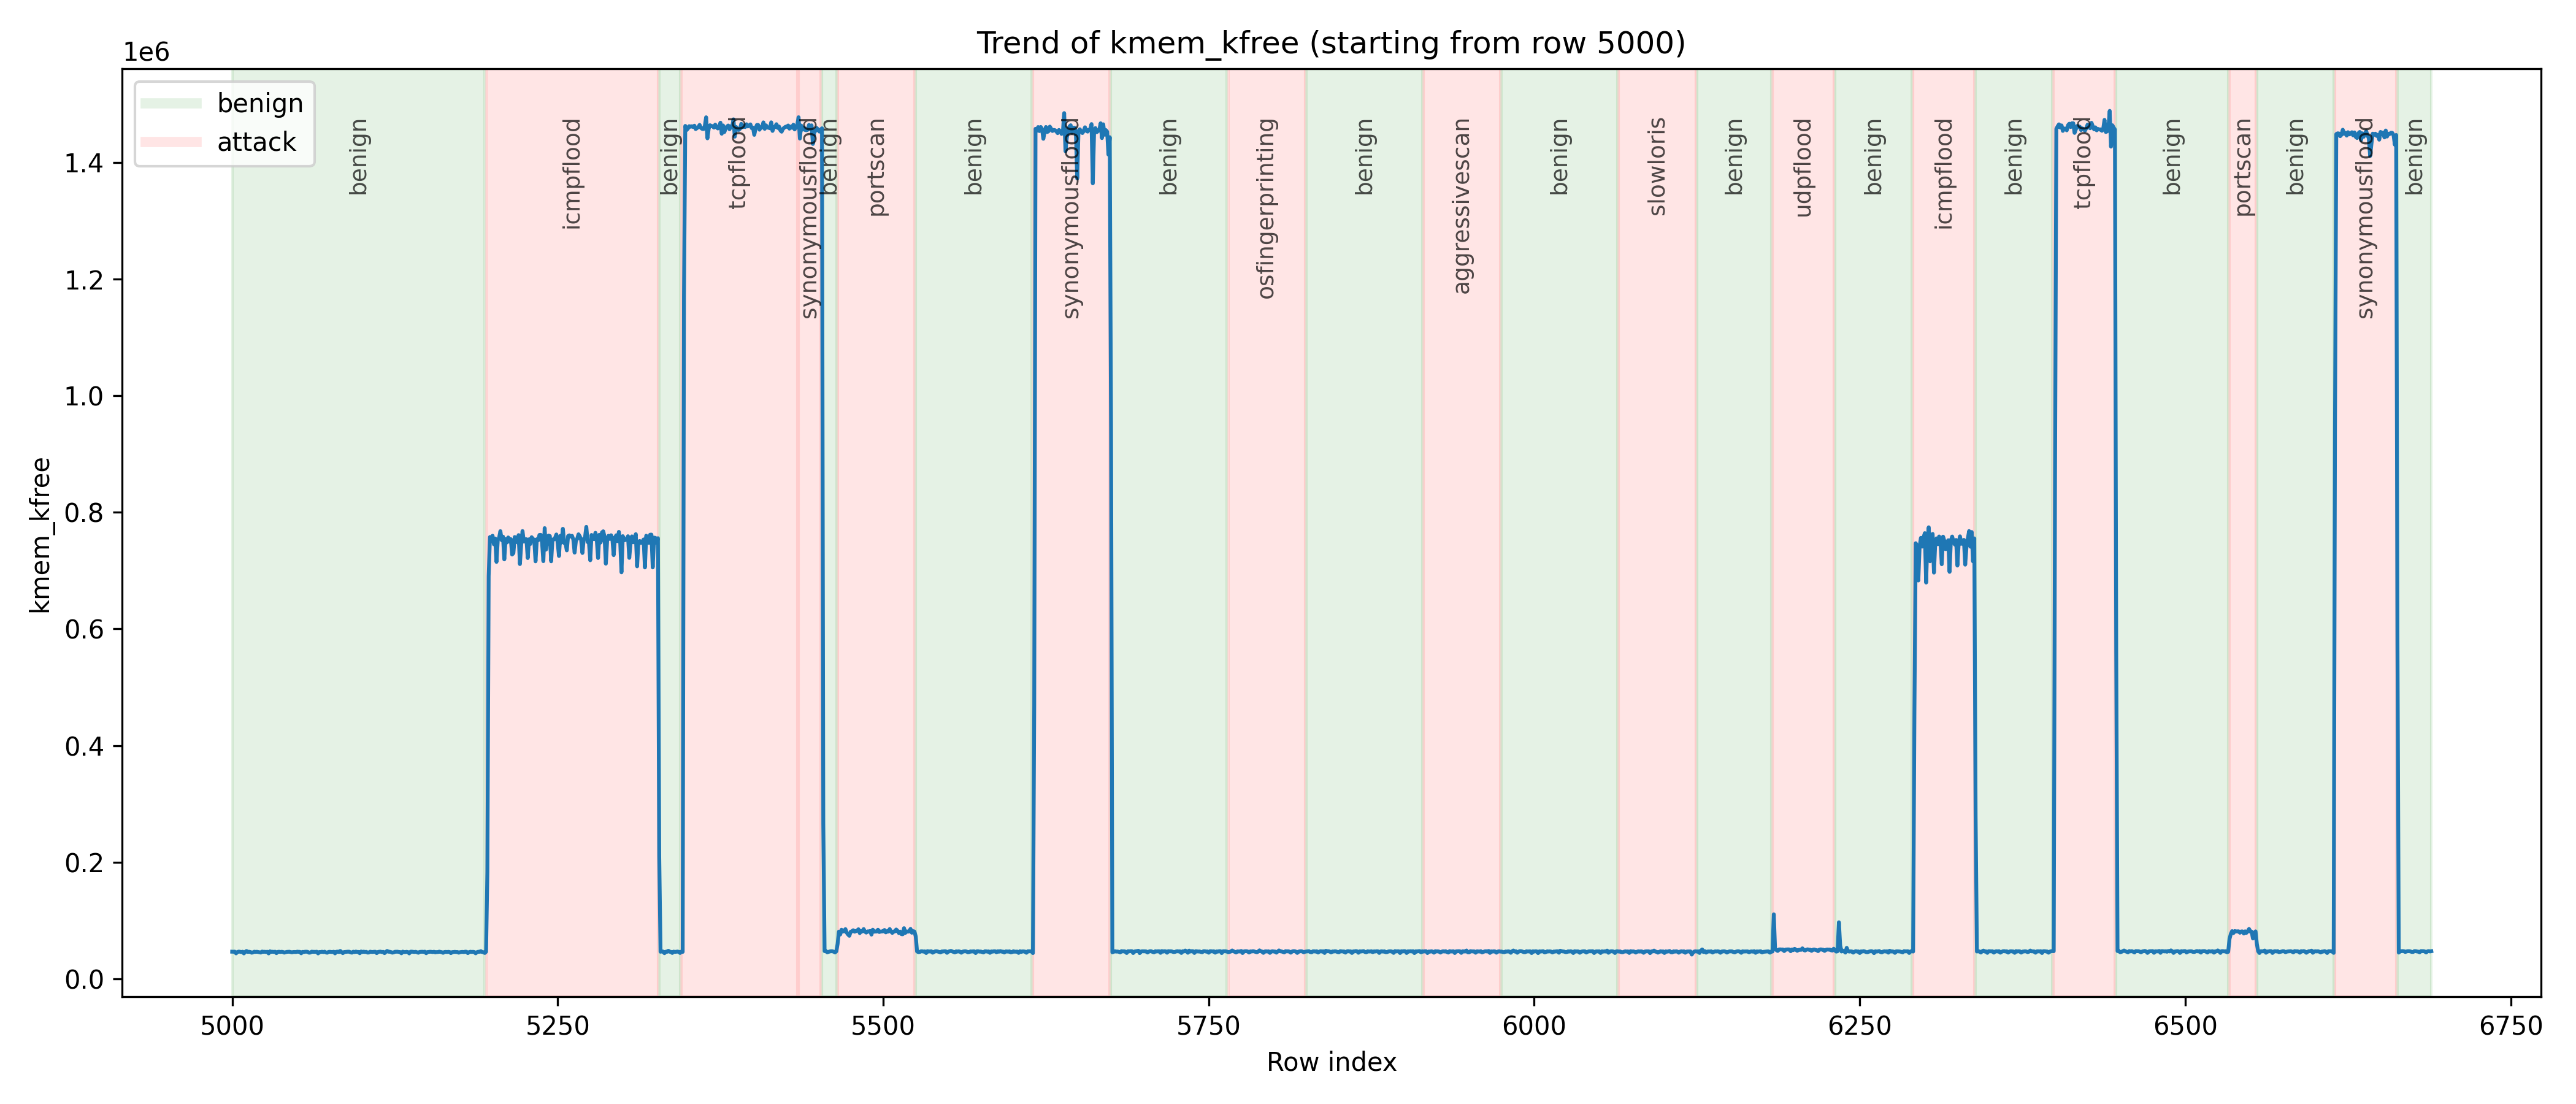
\includegraphics[width=1\textwidth]{pics/kmem_kfree.png}
  \vspace{-3mm} % Abstand manuell entfernen (anpassbar)
  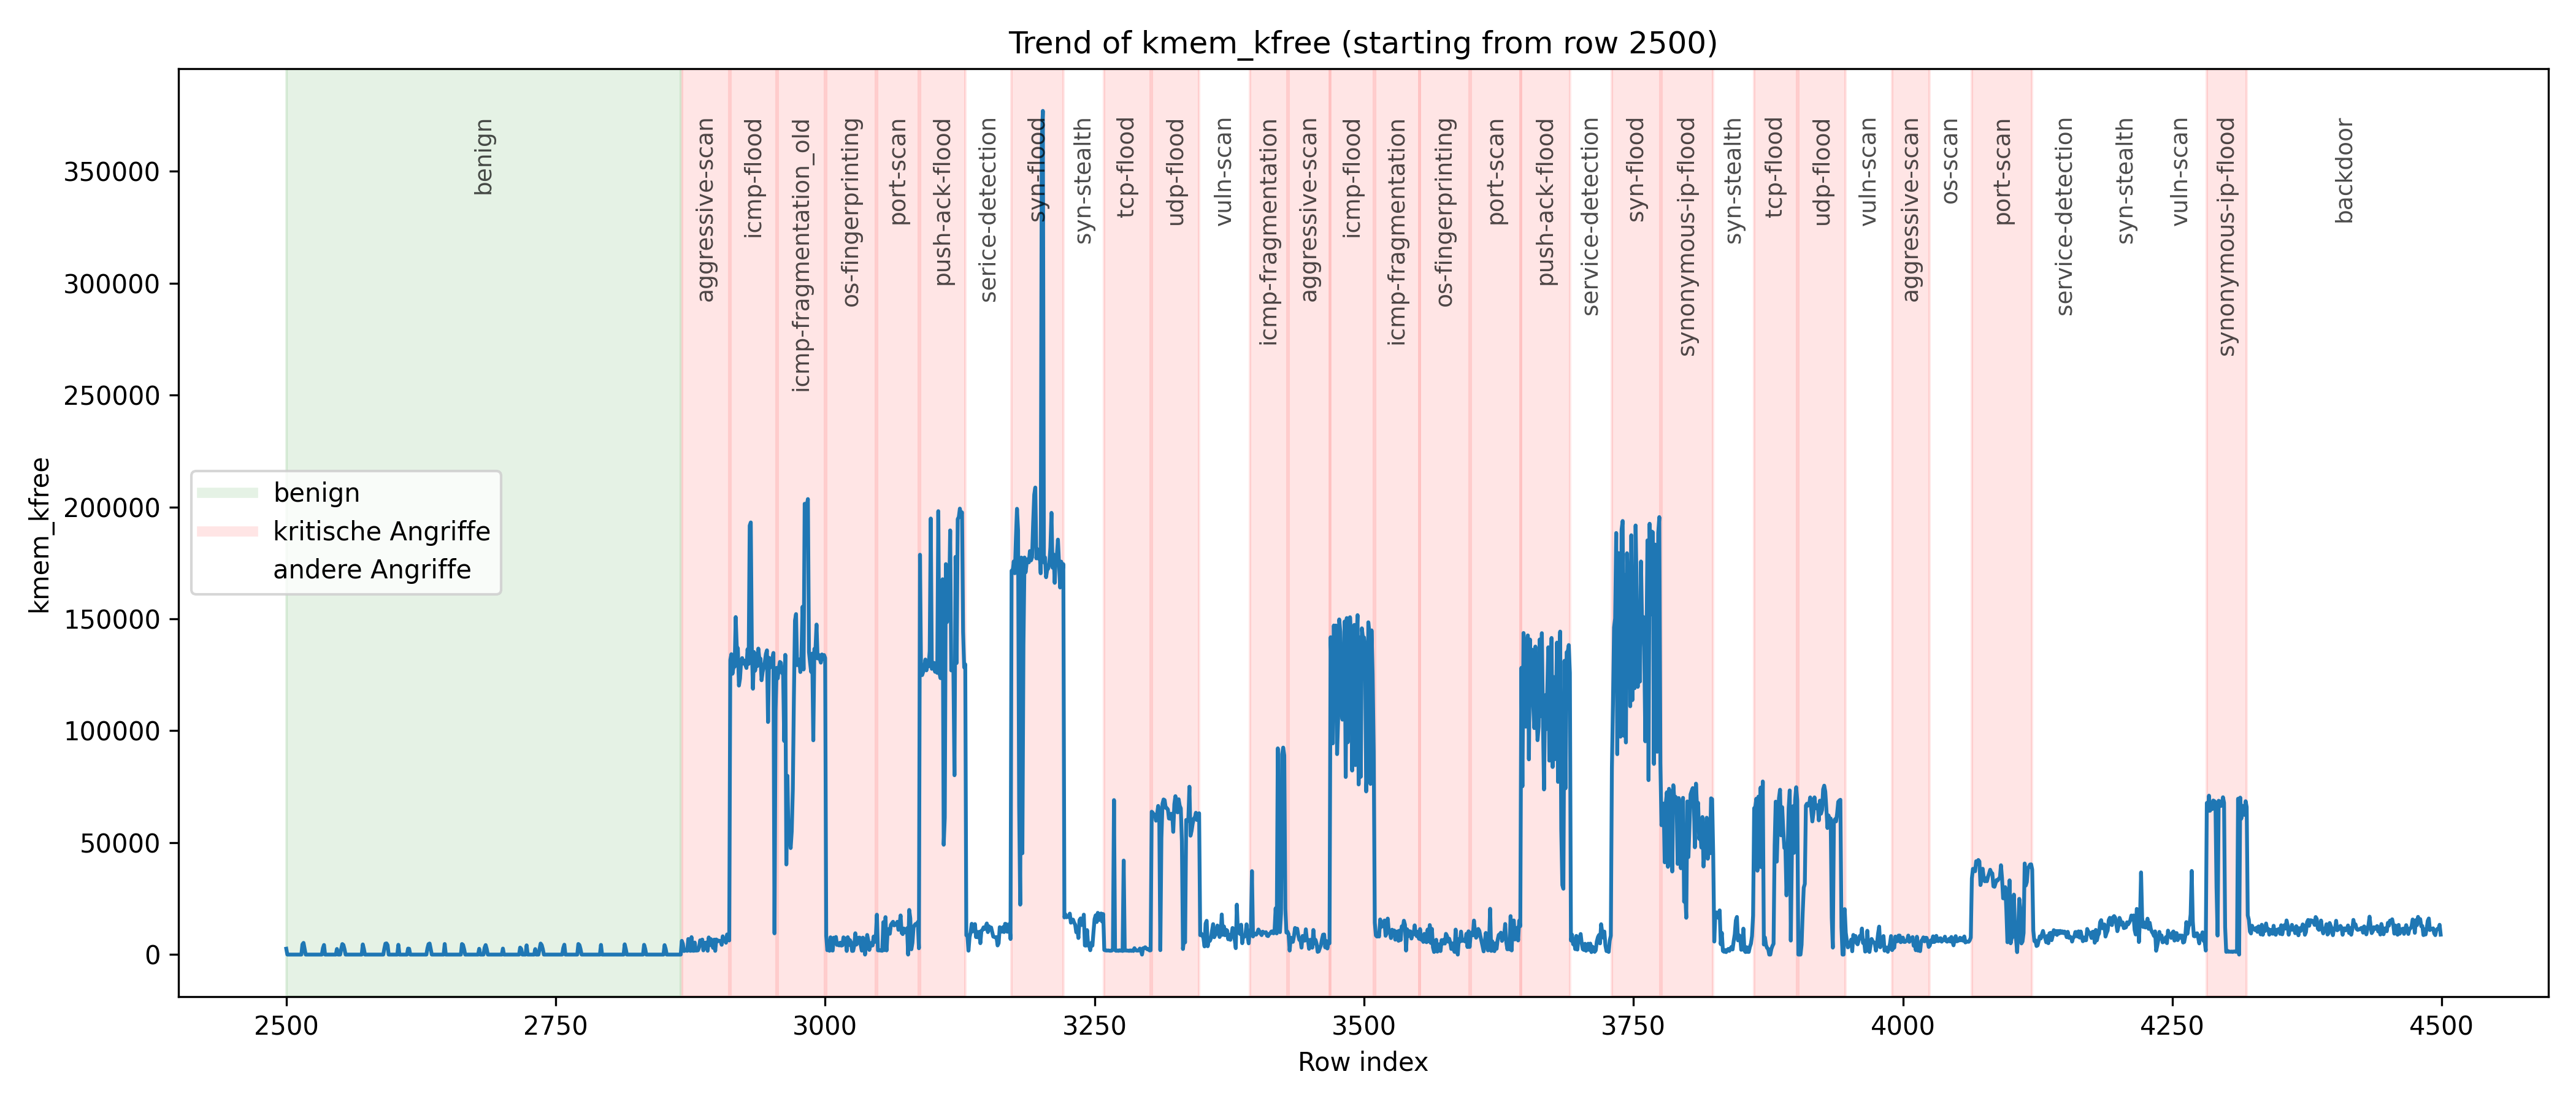
\includegraphics[width=1\textwidth]{pics/kmem_kfree_public.png}
  \caption{Comparison of \texttt{kmem-kfree} timelines: own dataset (top) and CICEVSE2024 dataset (bottom)}
  \label{fig:kmem_kfree_comparison}
\end{figure}
We observe similar peaks in both datasets, particularly during the flooding attacks, where the counter for \texttt{kmem\_kfree} increases noticeably. In our dataset, the resulting curve is cumulative, showing pronounced peaks corresponding to the attack phases. In contrast, the CICEVSE2024 dataset exhibits a more oscillating pattern, which is likely a result of different \texttt{perf} measurement flags. Specifically, their approach appears to monitor within a fixed time window, resetting the counter after each interval. This methodological difference leads to the observed oscillatory course in the public dataset, while the cumulative approach in our dataset amplifies peaks and produces a monotonically increasing curve.\\
\\
Therefore, we have sufficient data to train our models with minimal error values. Moreover, for the selected features from the paper \textit{Enhancing EV Charging Station Security Using a Multi-dimensional Dataset}~\cite{EV_Security}, we observe similar peaks and behavioral patterns in both attack and benign scenarios. This indicates a high degree of similarity between the datasets, further supporting the generalizability and validity of the selected features for anomaly detection.


\pagebreak
% ----------------------------------------------------------------------------------
% Kapitel: Feature selection 5
% ----------------------------------------------------------------------------------
\subsection{Data Preprocessing Steps}

As already mentioned, for the CICEVSE2024 dataset, it was only necessary to remove four rows containing \texttt{NaN} values to obtain clean and usable data for the initial processing step. \\

For the dataset generated from the experimental environment, the aim was first to include as much benign-status data as possible. Therefore, a PromQL request was made to retrieve monitoring data from a night when the environment was not used for other tests, as shown in Listing \ref{lst:prometheustocsv_scraper}. \\

Subsequently, the attacks were initiated to monitor the behavior of the HPC and kernel events in the environment under attack conditions, which can be seen in Listing \ref{lst:python_attack_script}.  
Table~\ref{tab:attacks} provides an overview of all attacks carried out during the experiment.

\begin{table}[H]
\centering
\begin{tabular}{|l|l|l|}
\hline
\textbf{Attack Type} & \textbf{Tool} & \textbf{Description / Parameters} \\
\hline
Slowloris          & Python script  & 500 sockets against target host \\
UDP-Flood          & hping3         & \texttt{--flood --udp -p 80} \\
ICMP-Flood         & hping3         & \texttt{--flood -1} \\
TCP-Flood          & hping3         & \texttt{--flood -p 80} \\
SYN-Flood          & hping3         & \texttt{--flood --rand-source -p 80} \\
Portscan           & nmap           & 1000 iterations, \texttt{-sT} scan \\
OS-Fingerprinting  & nmap           & 1000 iterations, \texttt{-O} scan \\
Aggressive-Scan    & nmap           & 1000 iterations, \texttt{-A} scan \\
\hline
\end{tabular}
\caption{Overview of executed attacks.}
\label{tab:attacks}
\end{table}

Using the generated log file, the correct attack intervals could be assigned to the dataset file for machine learning training and data analysis.  
Table~\ref{tab:intervals} shows the exact time periods used.

\begin{table}[H]
\centering
\begin{tabular}{|l|l|l|}
\hline
\textbf{Start Time} & \textbf{End Time} & \textbf{Attack Type} \\
\hline
2025-07-23 06:52:35 & 2025-07-23 07:07:35 & Slowloris \\
2025-07-23 07:27:35 & 2025-07-23 07:42:35 & UDP-Flood \\
2025-07-23 08:25:45 & 2025-07-23 08:47:50 & ICMP-Flood \\
2025-07-23 08:50:49 & 2025-07-23 09:05:49 & TCP-Flood \\
2025-07-23 09:05:49 & 2025-07-23 09:08:49 & SYN-Flood \\
2025-07-23 09:10:44 & 2025-07-23 09:20:44 & Portscan \\
2025-07-23 09:35:44 & 2025-07-23 09:45:44 & SYN-Flood \\
2025-07-23 10:00:44 & 2025-07-23 10:10:44 & OS-Fingerprinting \\
2025-07-23 10:25:44 & 2025-07-23 10:35:44 & Aggressive-Scan \\
2025-07-23 10:50:44 & 2025-07-23 11:00:44 & Slowloris \\
2025-07-23 11:10:21 & 2025-07-23 11:18:21 & UDP-Flood \\
2025-07-23 11:28:21 & 2025-07-23 11:36:21 & ICMP-Flood \\
2025-07-23 11:46:21 & 2025-07-23 11:54:21 & TCP-Flood \\
2025-07-23 12:08:55 & 2025-07-23 12:12:21 & Portscan \\
2025-07-23 12:22:21 & 2025-07-23 12:30:21 & SYN-Flood \\
\hline
\end{tabular}
\caption{Attack intervals during data collection.}
\label{tab:intervals}
\end{table}

These preprocessing steps enabled a meaningful exploratory data analysis, which allowed for the identification of key features for training machine learning models to achieve optimal results.  
This step is essential, as most models do not perform well with 900 or more features. This is also demonstrated in source \cite{EV_Security}, where the best results were achieved using only 11 to 20 key features. \\

Moreover, using too many features would lead to performance issues on the Raspberry Pi in the live system, as it would be required to query and process values for up to 900 features every 5 to 60 seconds.

% Insert figure demonstrating performance issues when querying 900 features

\input{content/chapter/6_Feature_Selection/6.2_key_feature_selection}
\subsection{Feature Selection Using Decision Trees}


\pagebreak
% ----------------------------------------------------------------------------------
% Kapitel: LSTM Architecutre 5
% ----------------------------------------------------------------------------------
\section{LSTM Architecture: Structure, Training, and Optimization}

\subsection{Structure and Functionality of the LSTM Architecture}
\subsection{Training Procedure and Validation Strategy}
\subsection{Parameter Configuration and Hyperparameter Optimization}

\pagebreak

% ----------------------------------------------------------------------------------
% Kapitel: Analysis and Evaluation 5
% ----------------------------------------------------------------------------------
\subsection{Experimental Setup and Evaluation Metrics}

To evaluate the model objectively and verify whether it correctly detects anomalies, this work follows a systematic approach. Clearly separated test data from the dataset \textit{CICEVSE2024} as well as from the dataset collected in the course of this work were used. In addition, the model was tested in a live environment with real-time detection.\\

The dataset \textit{CICEVSE2024} and the dataset collected for this work were already split into training and test data, as described in Chapter~7.1 \textit{LSTM Architecture and Preprocessing}. The test data was used to evaluate the model’s performance and consists of fixed time periods to ensure that the LSTM correctly utilizes its memory and detects attacks based on changes in the event data over time.\\

The trained LSTM model as well as the scaling parameters (StandardScaler) were exported and deployed for live classification on a resource-constrained Raspberry Pi system. Using Prometheus as a monitoring solution and a specially developed performance exporter (see Appendix~\pageref{code:perf_exporter}), measurement data could be provided at the desired interval.\\

To realistically test the model’s behavior, various attack patterns (e.g., flooding, scans, Slowloris) were executed in an automated manner with precise time logging (see Appendix~\pageref{code:xy}). This enabled a targeted analysis of the classification output during typical threat scenarios.\\

\textbf{Evaluation Metrics:} The quality of anomaly detection was assessed using established metrics for binary classification:
\begin{itemize}
    \item \textbf{Accuracy}: Proportion of correctly classified samples relative to the total number of samples.
    \item \textbf{Precision}: Proportion of actual attacks among all samples classified as attacks.
    \item \textbf{Recall}: Proportion of detected attacks among all actual attacks.
    \item \textbf{F1-Score}: Harmonic mean of Precision and Recall, particularly relevant for imbalanced classes.
    \item \textbf{Visualization}: Additionally, distribution and edge cases were illustrated using the Confusion Matrix, ROC Curve, and Precision-Recall Curve.
\end{itemize}

The focus, beyond the pure detection rate, was placed on the robustness of the model with respect to different types of attacks and possible data deviations during live operation.\\

These metrics serve as the foundation for the detailed result analysis in the following section and allow for a transparent evaluation of the practical applicability of the approach.

\subsection{Results of Anomaly Detection Using the Machine Learning Model}
\subsection{Visualization and Interpretation of Detected Anomalies}

% ----------------------------------------------------------------------------------
% Kapitel: Discussion 2
% ----------------------------------------------------------------------------------
\section{Discussion}


\pagebreak
% ----------------------------------------------------------------------------------
% Kapitel: Future Work 2
% ----------------------------------------------------------------------------------
\section{Conclusion/Future Work}
\pagebreak

% ----------------------------------------------------------------------------------------------------------
% Filter fuer Literatur und Quellen definieren
% ----------------------------------------------------------------------------------------------------------

\defbibheading{Literatur}{\section*{Literaturverzeichnis}} 
\defbibheading{Quellen}{\section*{Quellenverzeichnis}} 
  
\defbibfilter{Literatur}{\not\keyword{online}} 
\defbibfilter{Quellen}{\keyword{online}} 


% ----------------------------------------------------------------------------------------------------------
% Literatur
% ----------------------------------------------------------------------------------------------------------
\lhead{} 
\rhead{Literaturverzeichnis} 

\printbibliography[heading=Literatur,filter=Literatur] 

\pagebreak

% ----------------------------------------------------------------------------------------------------------
% Anhang
% ----------------------------------------------------------------------------------------------------------

\pagenumbering{Roman}
\setcounter{page}{1}
\lhead{Anhang \thesection}

\appendix
\section*{Anhang}

\label{app:perf_script}
\begin{lstlisting}[caption={Go script for performance monitoring via perf for Prometheus}, label={lst:perf-prometheus-exporter}]
package main
import (
	"fmt"
	"io/ioutil"
	"net/http"
	"os/exec"
	"strconv"
	"strings"
	"time"

	"gopkg.in/yaml.v2"
)

// Config represents the structure of the YAML configuration file.
// It includes high-level performance counters (HCP), software events (SW), and hardware events (HW).
type Config struct {
	HCP []string `yaml:"hcp"`
	SW  []string `yaml:"sw"`
	HW  []string `yaml:"hw"`
}

// Global variable to store the most recent performance data.
var perfData string

// getPerfData runs `perf stat` with the specified events for a short duration (0.1s)
// and returns the raw output as a string.
func getPerfData(events []string) (string, error) {
	eventList := strings.Join(events, ",")
	cmd := exec.Command("perf", "stat", "-e", eventList, "--", "sleep", "0.1")
	output, err := cmd.CombinedOutput()
	if err != nil {
		return "", err
	}
	return string(output), nil
}

// parsePerfData filters and extracts only the relevant lines from perf output,
// based on the provided list of events.
func parsePerfData(data string, events []string) string {
	lines := strings.Split(data, "\n")
	var result []string
	for _, line := range lines {
		for _, event := range events {
			if strings.Contains(line, event) {
				result = append(result, line)
				break
			}
		}
	}
	return strings.Join(result, "\n")
}

// formatForPrometheus converts the filtered performance data into Prometheus-compatible metrics format.
func formatForPrometheus(data string) string {
	lines := strings.Split(data, "\n")
	var result []string
	for _, line := range lines {
		parts := strings.Fields(line)
		if len(parts) >= 2 {
			// Clean up the metric name
			metricName := strings.ReplaceAll(parts[1], ".", "_")
			// metricName = strings.ReplaceAll(metricName, "-", "_")
			// Remove decimal points from the number and parse it
			metricValue := strings.ReplaceAll(parts[0], ".", "")
			if value, err := strconv.ParseFloat(metricValue, 64); err == nil {
				// Format value appropriately for Prometheus (integer or float)
				if value == float64(int(value)) {
					result = append(result, fmt.Sprintf("%s %d", metricName, int(value)))
				} else {
					result = append(result, fmt.Sprintf("%s %f", metricName, value))
				}
			}
		}
	}
	return strings.Join(result, "\n")
}

// metricsHandler handles HTTP requests and returns the formatted performance metrics.
func metricsHandler(w http.ResponseWriter, r *http.Request) {
	fmt.Fprintf(w, formatForPrometheus(perfData))
}

// chunkEvents splits the list of events into smaller chunks of a given size.
// This helps avoid issues with perf's limit on the number of simultaneous counters.
func chunkEvents(events []string, chunkSize int) [][]string {
	var chunks [][]string
	for i := 0; i < len(events); i += chunkSize {
		end := i + chunkSize
		if end > len(events) {
			end = len(events)
		}
		chunks = append(chunks, events[i:end])
	}
	return chunks
}

// validateEvent checks if a given performance event is available on the system by using `perf list`.
func validateEvent(event string) bool {
	cmd := exec.Command("perf", "list")
	output, err := cmd.CombinedOutput()
	if err != nil {
		fmt.Println("Error listing perf events:", err)
		return false
	}
	return strings.Contains(string(output), event)
}

func main() {
	// Load the YAML configuration file
	config := Config{}
	data, err := ioutil.ReadFile("config.yml")
	if err != nil {
		fmt.Println("Error reading config file:", err)
		return
	}
	err = yaml.Unmarshal(data, &config)
	if err != nil {
		fmt.Println("Error parsing config file:", err)
		return
	}

	// Validate and collect all available events from the config
	var validEvents []string
	for _, event := range append(config.HCP, config.SW...) {
		if validateEvent(event) {
			validEvents = append(validEvents, event)
		}
	}
	for _, event := range config.HW {
		if validateEvent(event) {
			validEvents = append(validEvents, event)
		}
	}

	// Split the events into manageable chunks (TODO: dynamically adjust based on CPU performance)
	eventChunks := chunkEvents(validEvents, 6)

	// Start a background goroutine to periodically collect performance data
	go func() {
		for {
			var allPerfData []string
			for _, chunk := range eventChunks {
				data, err := getPerfData(chunk)
				if err != nil {
					fmt.Println("Error:", err)
					allPerfData = append(allPerfData, "Error fetching data")
				} else {
					allPerfData = append(allPerfData, parsePerfData(data, chunk))
				}
			}
			// Combine data from all chunks into one string for Prometheus export
			perfData = strings.Join(allPerfData, "\n")
			time.Sleep(100 * time.Millisecond)
		}
	}()

	// Start the HTTP server that exposes the `/metrics` endpoint for Prometheus scraping
	http.HandleFunc("/metrics", metricsHandler)
	fmt.Println("Starting server on :9011")
	if err := http.ListenAndServe(":9011", nil); err != nil {
		fmt.Println("Error starting server:", err)
	}
}
\end{lstlisting}

\begin{lstlisting}[caption={Python script for scraping performance monitoring from Prometheus into an csv file}, label={lst:prometheustocsv_scraper}]
import requests
import csv
from datetime import datetime, timedelta
from collections import defaultdict
import numpy as np

from config_allevents import FEATURES

PROMETHEUS_URL = "http://192.168.1.25:9090"
STEP = "10"  # seconds
CHUNK_HOURS = 2

start_time = datetime.fromisoformat("2025-07-22T18:00:00.000000")
end_time = datetime.fromisoformat("2025-07-23T14:40:00.000000")

def build_chunks(start, end, chunk_hours):
    chunks = []
    chunk_delta = timedelta(hours=chunk_hours)
    current_start = start
    while current_start < end:
        current_end = min(current_start + chunk_delta, end)
        chunks.append((
            current_start.isoformat("T") + "Z",
            current_end.isoformat("T") + "Z"
        ))
        current_start = current_end
    return chunks

def query_metric_chunked(metric, chunks):
    all_results = []
    for chunk_start, chunk_end in chunks:
        url = f"{PROMETHEUS_URL}/api/v1/query_range"
        params = {
            "query": metric,
            "start": chunk_start,
            "end": chunk_end,
            "step": STEP,
        }
        response = requests.get(url, params=params)
        response.raise_for_status()
        all_results.extend(response.json()["data"]["result"])
    return all_results

def main():
    chunks = build_chunks(start_time, end_time, CHUNK_HOURS)
    data = defaultdict(dict)
    timestamps = set()
    values_dict = {}
    metric_query_map = {}

    for feat in FEATURES:
        prom_name = feat.replace("-", "_")
        url = f"{PROMETHEUS_URL}/api/v1/query"
        hit = False

        # 1. sum(prom_name) abfragen
        query = f"sum({prom_name})"
        params = {'query': query}
        try:
            resp = requests.get(url, params=params)
            resp.raise_for_status()
            results = resp.json()['data']['result']
            if results:
                value = float(results[0]['value'][1])
                values_dict[feat] = value
                metric_query_map[feat] = query
                hit = True
        except Exception:
            pass

        if hit:
            continue

        # 2. sum(perf_prom_name) abfragen
        prom_name_perf = 'perf_' + prom_name
        query = f"sum({prom_name_perf})"
        params = {'query': query}
        try:
            resp = requests.get(url, params=params)
            resp.raise_for_status()
            results = resp.json()['data']['result']
            if results:
                value = float(results[0]['value'][1])
                values_dict[feat] = value
                metric_query_map[feat] = query
                hit = True
        except Exception:
            pass

    values_array = []
    feature_names_for_array = []

    for feat in FEATURES:
        feature_names_for_array.append(feat)
        values_array.append(values_dict.get(feat, np.nan))

    for feat, querystr in metric_query_map.items():
        results = query_metric_chunked(querystr, chunks)
        for series in results:
            for timestamp, value in series["values"]:
                ts = datetime.utcfromtimestamp(float(timestamp)).isoformat()
                data[ts][feat] = value
                timestamps.add(ts)

    sorted_timestamps = sorted(timestamps)

    all_columns = list(FEATURES)

    with open("evse_metrics_wide.csv", "w", newline="") as f:
        writer = csv.writer(f)
        header = ["timestamp"] + all_columns
        writer.writerow(header)
        for ts in sorted_timestamps:
            row = [ts] + [data[ts].get(col, "") for col in all_columns]
            writer.writerow(row)

if __name__ == "__main__":
    main()
\end{lstlisting}

\begin{lstlisting}[caption={Python script for automatet attacks and storage of the timestamps}, label={lst:python_attack_script}]
import subprocess
import time
from datetime import datetime

commands = [
    ("Slowloris", ["python3", "slowloris.py", "192.168.1.25", "-s", "500"]),
    ("UDP Flood", ["sudo", "hping3", "--flood", "--udp", "-p", "80", "192.168.1.25"]),
    ("ICMP Flood", ["sudo", "hping3", "--flood", "-1", "192.168.1.25"]),
    ("TCP Flood", ["sudo", "hping3", "--flood", "-p", "80", "192.168.1.25"]),
    ("Synonymous Flood", ["sudo", "hping3", "--flood", "--rand-source", "-p", "80", "192.168.1.25"]),
    ("Portscan", ["bash", "-c", "for i in {1..1000}; do sudo nmap -sT 192.168.1.25; sleep 1; done"]),
    ("OS Fingerprinting", ["bash", "-c", "for i in {1..1000}; do sudo nmap -O 192.168.1.25; sleep 1; done"]),
    ("Aggressive Scan", ["bash", "-c", "for i in {1..1000}; do sudo nmap -A 192.168.1.25; sleep 1; done"]),
]

LOG_FILE = "timestamp_attacks.txt"
RUN_TIME = 15 * 60      # 15 Minuten
BREAK_TIME = 20 * 60    # 20 Minuten

def log_msg(msg):
    with open(LOG_FILE, "a") as f:
        f.write(msg + "\n")

while True:
    for name, cmd in commands:
        start_time = datetime.now()
        print(f"Starte {name}: {' '.join(cmd)}")
        log_msg(f"Start: {start_time.strftime('%Y-%m-%d %H:%M:%S')} - Angriff: {name} - Befehl: {' '.join(cmd)}")
        try:
            proc = subprocess.Popen(cmd)
            proc.wait(timeout=RUN_TIME)
            note = "Erfolgreich beendet"
        except subprocess.TimeoutExpired:
            proc.terminate()
            try:
                proc.wait(10)
            except Exception:
                proc.kill()
            note = "Nach 15 Minuten abgebrochen"
        end_time = datetime.now()
        log_msg(f"Ende: {end_time.strftime('%Y-%m-%d %H:%M:%S')} ({note})")
        log_msg("Pause startet jetzt.\n")
        time.sleep(BREAK_TIME)
\end{lstlisting}


\phantomsection
\addcontentsline{toc}{section}{Anhang}
\addtocontents{toc}{\vspace{-0.5em}}

content des beigefügten Datenträgers:
\begin{itemize}
  \item $\ldots$
  \item $\ldots$
\end{itemize}

\section{Domändenmodell}
Ein toller Anhang, der nicht nur als \glqq{}\emph{Müllhalde}\grqq{} genutzt wird, sondern in dem Bilder und contente auch mit eigenen Worten erklärt werden und den man auch für sich alleine lesen kann. Es sollten auch Referenzen auf die zugehörige ausführliche Behandlung im Hauptteil inklusive Seitenangabe mit $\backslash$\texttt{pageref} gegeben werden.

\subsection*{Screenshot}
\label{app:screenshot}
Unterkategorie, die nicht im contentsverzeichnis auftaucht.

\appendix


\pagebreak




\end{document}